% Options for packages loaded elsewhere
\PassOptionsToPackage{unicode}{hyperref}
\PassOptionsToPackage{hyphens}{url}
%
\documentclass[
]{book}
\usepackage{amsmath,amssymb}
\usepackage{lmodern}
\usepackage{iftex}
\ifPDFTeX
  \usepackage[T1]{fontenc}
  \usepackage[utf8]{inputenc}
  \usepackage{textcomp} % provide euro and other symbols
\else % if luatex or xetex
  \usepackage{unicode-math}
  \defaultfontfeatures{Scale=MatchLowercase}
  \defaultfontfeatures[\rmfamily]{Ligatures=TeX,Scale=1}
\fi
% Use upquote if available, for straight quotes in verbatim environments
\IfFileExists{upquote.sty}{\usepackage{upquote}}{}
\IfFileExists{microtype.sty}{% use microtype if available
  \usepackage[]{microtype}
  \UseMicrotypeSet[protrusion]{basicmath} % disable protrusion for tt fonts
}{}
\makeatletter
\@ifundefined{KOMAClassName}{% if non-KOMA class
  \IfFileExists{parskip.sty}{%
    \usepackage{parskip}
  }{% else
    \setlength{\parindent}{0pt}
    \setlength{\parskip}{6pt plus 2pt minus 1pt}}
}{% if KOMA class
  \KOMAoptions{parskip=half}}
\makeatother
\usepackage{xcolor}
\IfFileExists{xurl.sty}{\usepackage{xurl}}{} % add URL line breaks if available
\IfFileExists{bookmark.sty}{\usepackage{bookmark}}{\usepackage{hyperref}}
\hypersetup{
  pdftitle={Pig Science - Part Breeding},
  pdfauthor={Peter von Rohr},
  hidelinks,
  pdfcreator={LaTeX via pandoc}}
\urlstyle{same} % disable monospaced font for URLs
\usepackage{longtable,booktabs,array}
\usepackage{calc} % for calculating minipage widths
% Correct order of tables after \paragraph or \subparagraph
\usepackage{etoolbox}
\makeatletter
\patchcmd\longtable{\par}{\if@noskipsec\mbox{}\fi\par}{}{}
\makeatother
% Allow footnotes in longtable head/foot
\IfFileExists{footnotehyper.sty}{\usepackage{footnotehyper}}{\usepackage{footnote}}
\makesavenoteenv{longtable}
\setlength{\emergencystretch}{3em} % prevent overfull lines
\providecommand{\tightlist}{%
  \setlength{\itemsep}{0pt}\setlength{\parskip}{0pt}}
\setcounter{secnumdepth}{5}
\usepackage{booktabs}
\usepackage{amsthm}
\usepackage{float}
\usepackage{graphicx}
\makeatletter
\def\thm@space@setup{%
  \thm@preskip=8pt plus 2pt minus 4pt
  \thm@postskip=\thm@preskip
}
\makeatother
\ifLuaTeX
  \usepackage{selnolig}  % disable illegal ligatures
\fi
\usepackage[]{natbib}
\bibliographystyle{plainnat}

\title{Pig Science - Part Breeding}
\author{Peter von Rohr}
\date{2022-04-26}

\begin{document}
\maketitle

{
\setcounter{tocdepth}{1}
\tableofcontents
}
\hypertarget{preface}{%
\chapter*{Preface}\label{preface}}
\addcontentsline{toc}{chapter}{Preface}

The material presented here is in part based on course notes from \citep{Goetz2014}. The main goal of this part of the course is to transport a clear view of different concepts in the context of the pig breeding program in Switzerland. After this course, the students have a clear understanding of the terms

\begin{itemize}
\tightlist
\item
  livestock breeding
\item
  livestock production and
\item
  animal husbandry
\end{itemize}

The main focus of this part of the course will be on different aspects that are related to a breeding program in general. The different types of breeding programs will be characterized. Furthermore, the components of a livestock breeding with a scientific foundation and a focus on economic objectives. The scientific foundation is important, because we want to evaluate or to measure the success of our breeding program and this is only possible, if the breeding program is built on a scientific foundation. Also the economic objective simplifies the evaluation of a given breeding program. As a consequence, an economic objective allows to compare different breeding programs.

\hypertarget{gel-intro}{%
\chapter{Introduction}\label{gel-intro}}

\hypertarget{gel-intro-terminology}{%
\section{Terminology}\label{gel-intro-terminology}}

The terms \textbf{livestock breeding} or \textbf{breeding} in general are used ambiguously. Both terms are associated with many different meanings. Most people use the term \emph{livestock breeder} when they effectively mean \emph{livestock owner} or \emph{livestock producer}. From a scientific point of view \textbf{livestock breeders} use the tools of \textbf{selection} and \textbf{mating} to obtain offspring animals which are closer to a certain breeding goal compared to the parent generation. In pet breeding, individual breeders are known to use these tools in order to realize their special breeding goals. The special circumstances of pet breeding which is mostly used for cats and dogs are not further described in these course notes. When we talk about \textbf{livestock}, we mean farm animals such as cattle, pigs, sheeps or goats.

\hypertarget{gel-intro-background}{%
\section{Background}\label{gel-intro-background}}

Livestock breeders are also known to follow individual breeding goals. Due to some special circumstances in reproduction biology of livestock which are long generation intervals and low numbers of offspring per mating, have led breeders to recognize the need for gathering their efforts in breeding associations. Initially breeding organisations were responsible for the herdbook which was a central registry of all animals that were owned by members of the breeding organisation. Breeding organisation also helped their members to buy and to sell their animals.

\begin{figure}[H]
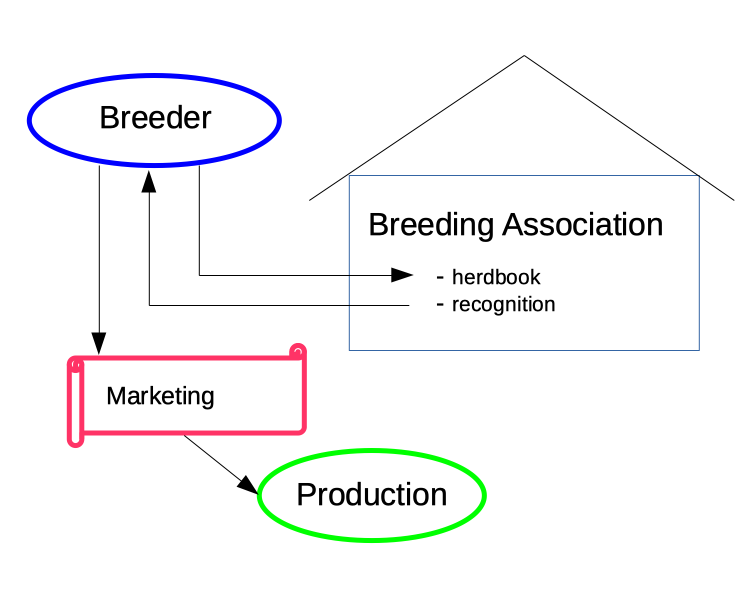
\includegraphics[width=11cm]{odg/breedingassociation} \caption{Schematic Representation Of A Breeding Organisation}\label{fig:breedingassociation}
\end{figure}

In the middle of the \(19^{th}\) century, Switzerland was transformed from an agricultural society into an industrial society. With the invention of modern railway systems, costs for transportation was lowered significantly. As a consequence, food production in Switzerland dropped and many nutrients were imported. This development was not recognized until the beginning of the first world war. Closed borders and many resources bound in military services lead to a big crisis of food supplies. As a result of this crisis, the federal government started to introduce important laws to regulate breeding goals in Swiss livestock breeding. The initial versions of these laws were clearly directed towards an increase in performance of livestock animals. The most important federal regulation concerning livestock breeding is the so-called ``Tierzuchtverordnung'' \citep{Bundesrat2012}. This regulation contains requirements for the recognition of breeding organisation. It also lists the amount of subsides that the breeding organisations are entitled to receive for the different services. In the current version of the regulation, these subsidies are tied to explicitly mentioned performance tests and recordings. An additional requirement is a scientifically recognized procedure to predict breeding values. In 2014 the federal government started a revision process of this legislation. Some of the results of this revision process is summarized in a document entitled ``Tierzucht Strategie 2030'' \citep{Lehmann2018}. Depending on the final outcome of this revision process, the landscape of breeding organisations is expected to change in the future.

Besides the federal regulation as a major driving force for livestock breeding in Switzerland, the progress in reproduction biology with the introduction of artificial insemination and the new possibilities of the applications of molecular biology techniques such as the cheap and effective genotyping of large numbers of breeding animals has had an important influence on the progress of livestock populations. Originally artificial insemination was introduced for hygienic reasons to prevent the spread of sexually transmitted diseases. The use of modern technologies led to the disappearance of locally rooted livestock breeds for breeds with higher performances.

\hypertarget{gel-intro-breedingvsproduction}{%
\section{Breeding Versus Production}\label{gel-intro-breedingvsproduction}}

The distinction between \textbf{livestock breeding} and \textbf{production} is important because both activities may have goals and requirements which can be contradictory. The term \emph{production} stands for the use of livestock animals to generate products which are marketable and can be sold to the nutrition industry. Therefore we have to emphasize that requirements and goals are entirely determined by the buyers of nutrition products. From the point of view of the producer, the whole production process has to follow the rules given by farm business economics. In short, production processes are only maintained when they are profitable. This means the revenue obtained from selling the products are larger than the costs generated by the production process.

In livestock breeding additional requirements given by the breeding goal and the aim to improve livestock animals of all member farms of a breeding association on a genetic level must be considered. But a livestock breeding farm has the opportunity to generate additional revenues when breeding animals can be sold to other farms. Conflicts between requirements of breeding and production often arise when it comes to the question how valuable older animals are. From the perspective of a producer, old animals are the most valuable. Because they have covered their costs for raising them with their live-long generation of revenues. For a livestock breeder it is exactly the other way around. For the improvement of a population on the genetic level, the youngest animals are the most valuable. Because the genetic potential of the youngest animals is expected to be the highest.

\hypertarget{gel-intro-summary}{%
\section{Summary}\label{gel-intro-summary}}

In summary of this chapter, it is clear that in the context of these course notes, a livestock breeder is a person who is a member of a breeding organisation. A livestock breeder is together with his or her livestock herd part of the breeding program. The breeding program states a breeding goal and the breeder with his membership subscribes to follow with his or her herd the breeding goal defined in the breeding program. Based on that description of a livestock breeder, it becomes clear that milk producer is not a dairy cattle breeder and a pork producer is not a pig breeder.

In this course, the application of predicted breeding values in the context of a breeding program is introduced. The aim of the breeding program is to improve the livestock animals with respect to the breeding goal.

\hypertarget{gel-bprog}{%
\chapter{Breeding Programs}\label{gel-bprog}}

\hypertarget{gel-bprog-intro}{%
\section{Introduction}\label{gel-bprog-intro}}

As mentioned in chapter \ref{gel-intro} applied prediction of breeding values is an integral part of breeding programs. Figure \ref{fig:bprogdiag} shows the connection between the different parts of a breeding program.

\begin{figure}[H]
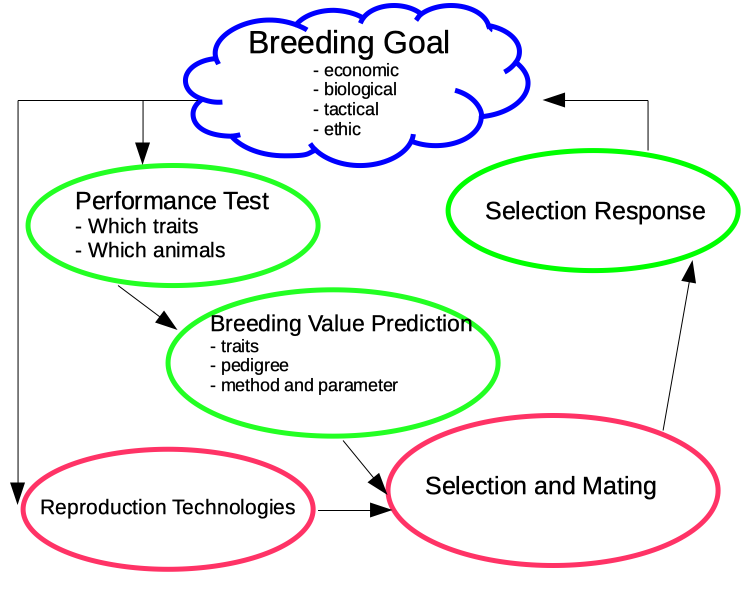
\includegraphics[width=11cm]{odg/bprogdiag} \caption{Connection Between Parts Of A Breeding Program}\label{fig:bprogdiag}
\end{figure}

The design process and the implementation of a breeding program are determined by the following two questions.

\begin{enumerate}
\def\labelenumi{\arabic{enumi}.}
\tightlist
\item
  Which goals should be achieved with a breeding program?
\item
  What types of measures should be used to achieve the breeding goal?
\end{enumerate}

In both questions the breeding goal is a central point and hence in order to be able to plan and to implement a breeding program, it is an absolute requirement to define a breeding goal. Breeding goals can be defined on different levels. For example, breeding goals can be

\begin{itemize}
\tightlist
\item
  \emph{economic}
\item
  \emph{biological}
\item
  \emph{ethical} or
\item
  \emph{tactical}
\end{itemize}

Economic breeding goals are focusing on the profit obtained by livestock breeding. Biological goals are used when traits do not have any marketable value. In cattle breeding, biological goals are applied for secondary traits\footnote{Examples of such traits are health traits, conformation or longevity.}. Ethical breeding goals are a more recent development. Their main focus is the prevention of phenotypes which do not allow the animals to lead a life that is free of pain and other health related restrictions. In some cases breeders might use tactical goals to stay in business which would not be justified by economic reasons.

There exist two types of breeding programs.

\begin{itemize}
\tightlist
\item
  breeding programs which focus on \textbf{selection response}
\item
  breeding programs in which the ability to sell breeding product and services is of central importance.
\end{itemize}

At first sight, one could think that all breeding programs are focusing on the achievement of a certain amount of selection response. Despite that it is still important to make this differentiation. The first type of breeding goals can mainly be observed in countries with scarce resources for human nutrition and with a restricted offer for animal food\footnote{Such conditions could also be observed in Europe during the first half of the \(20^th\) century.}. In such countries there is no infrastructure and the focus of livestock breeding is to use the available resources as efficiently as possible. This is only possible via the achievement of selection response. The first type of breeding programs can also be observed in countries with large herds or within private companies which run their own breeding programs. For such large farms or companies, their business success depends on the realization of selection response. Examples where such breeding programs can be observed are large beef cattle farms in Australia or Argentina or in large companies in pig breeding or in chicken breeding. In cattle breeding this type of development is only at an early stage. But large companies in the area of artificial insemination (AI) start to take a dominating role in the breeding business.

The second category of breeding programs can be observed in cattle breeding and pig breeding of developed countries. In this situation, only few farms and few AI companies determine the breeding program. The business success of these few companies is more important than the realization of selection response of the population. Selection response is still desirable but only as far as it helps for maximizing the profit of the few important companies. The difference between the two types of breeding programs is only very small, but it is important to realize that this difference does exist.

\hypertarget{gel-bprog-parts}{%
\section{Parts Of A Breeding Program}\label{gel-bprog-parts}}

Figure \ref{fig:bprogdiag} shows the parts of a breeding program. The design of a breeding program starts with the definition of a breeding goal. The performance testing, the prediction of breeding values and the measurement of the selection response are parts of the information centered aspect of the breeding program (shown in green). The implementation parts consisting of reproduction technologies, selection and mating are displayed in red.

\hypertarget{gel-bprog-perftest}{%
\subsection{Performance Testing}\label{gel-bprog-perftest}}

Serious livestock breeding is always based on data. These data are used directly as selection criteria or they are used as input for predicting breeding values. The accuracy of the collected data determines the quality of the derived parameters such as heritability and predicted breeding values. As a consequence of that, as much data should be collected for every animal in the population. This cannot be done because it is too expensive. Therefore every breeding organisation has to optimize between the amount of data collected and the costs that are occurring for the data recording activities.

Existing data recording activities were often started for reasons that are not related to livestock breeding. The following list gives a few examples.

\begin{itemize}
\tightlist
\item
  milk sample testing was started for reasons of quality assurance in milk industry companies
\item
  station based testing in pig breeding was introduced to make the observed performances comparable
\item
  own performance records of animals are still the most important source of information
\item
  in dairy cattle before the introduction of genomic selection, progeny testing was the most important source of information for bulls in traits that are only expressed in female offsprings.
\end{itemize}

The performance testing programs determine at which time point and for which animals which types of data are available. The length of the generation interval does have an influence on when certain traits which are expressed only in one sex can be observed.

\hypertarget{gel-bprog-classperftest}{%
\subsubsection{Classification of Performance Tests}\label{gel-bprog-classperftest}}

Performance tests can be classified according to the place where the test takes place. The two main types are \textbf{station tests} and \textbf{field tests}. Stations tests allow for more standardized testing environments and for the collection of more traits per tested animal. In many cases testing stations are associated with or have their own research laboratories in which research about new traits is conducted. Testing stations are cost intensive and some people have doubts about the generalizability of station test results to the more general conditions in the field.

Field testing are more cost efficient and happen under field conditions. The introduction of BLUP animal models to predict breeding values allows for the simultaneous estimation of environmental effects together with the prediction of breeding values. Hence a constant and controllable testing environment has lost its justification. Field testing can be more vulnerable to special treatments of selection candidates.

In practical livestock breeding whenever possible data from testing stations and from field tests are combined to make optimal use of the collected data to provide predictions of breeding values with maximal accuracy. This is certainly the case in pig breeding since the late 1990s. In cattle breeding periodically returning experiments with station testing herds are performed. In the 1990s there were several testing herds using multiple ovulation and embryo transfer (MOET) technologies. More recently several experiments with mixed forms of station and field testing were started. The new types of membership forms of the large dairy cattle breeding organisations can also be viewed as such mixed performance testing forms.

A different classification criterion for performance tests are the relationship between the selection candidate and the tested animals. Based on that criterion the following tests can be differentiated:

\begin{itemize}
\tightlist
\item
  \textbf{own performance} test: performance of the selection candidate is directly measured
\item
  \textbf{sib} test: tested animals and selection candidate are full- or half-sibs
\item
  \textbf{progeny} test: selection candidate is a parent of the tested animals.
\end{itemize}

\hypertarget{gel-bprog-perftesttrait}{%
\subsubsection{Traits}\label{gel-bprog-perftesttrait}}

In a breeding program performance tests should be done for the most important traits. To be able to include a trait in a performance test, the following requirements must be met.

\begin{itemize}
\tightlist
\item
  measurable with high accuracy
\item
  economically important
\item
  sufficiently large genetic variance and reasonable heritability
\item
  measurement procedure should have high repeatability
\item
  measurement procedure must be unbiased with respect to different external factors
\item
  measured traits should have as closely related to physiological expression of trait of interest
\item
  whenever possible traits should be measure and not subjectively assessed
\end{itemize}

Certain traits are too expensive to measure directly. In this cases \textbf{auxillary traits} are used. Auxiliary traits must be easy and efficient to measure and must be closely connected to the trait of interest. Examples of auxiliary traits are back-fat thickness in pigs used as proxy trait for meatiness. In dairy cattle somatic cell counts are used as a proxy for mastitis. When using auxiliary or proxy traits, one has to periodically verify the connection between the proxy and the trait of interest. Because selection is a dynamic process connections between traits are subject to changes.

\hypertarget{gel-bprog-predbv}{%
\subsection{Prediction Of Breeding Values}\label{gel-bprog-predbv}}

The majority of the active breeding programs use predicted breeding values. In Switzerland, federal regulations prescribe the process of predicting breeding values in order to receive subsidies for the breeding program. The predictions should correct for the environmental factors. Especially when considering traits with low heritability, prediction of breeding values using a BLUP based model is a must.

The recording of the phenotypic measurements during the performance testing is often much more expensive than the prediction of the breeding values. This makes it clear that only the best methods should be used to evaluate the precious data. Data evaluations on a routine basis were only made possible by the availability of cheap computing power. As a consequence of that the big performance gains in livestock animals did run parallel to the massive increase of cheap computing power.

The frequency how often breeding values are predicted depends on the species. In cattle breeding breeding values are predicted only three times per year. In pig breeding some evaluations are done every night. Pigs have much shorter generation intervals and therefore the cycle where new information about selection candidates arrive is much shorter compared to cattle. The duration of a lactation in cattle is much longer and hence the frequency with which new information arrives is smaller compared to pigs. With new technologies such as robot milking systems which allow for much more frequent data sampling and with evaluation methods that are based on daily milk yield and no longer on lactation yields, this difference between the species is decreasing. From the point of view of genetic evaluation, we have to note that more frequent evaluations cannot be done with the same amount of manual input compared to less frequent evaluations.

\hypertarget{gel-bprog-reprotech}{%
\subsection{Reproduction Technologies}\label{gel-bprog-reprotech}}

The introduction of reproduction technologies in livestock breeding has been responsible for the massive selection response since the \(20^{th}\) century. Artificial insemination (AI) in cattle and pigs have almost removed the limit for the number of progeny per sire. For all species where AI is used the prediction of breeding values has massively improved. The use of sires across different farms connects the animals on the different farms on a genetic level. This leads to a better separation of genetic effects from environmental factors.

Future developments are focusing more on reproduction technologies for dams. Embryo transfer increases the number of progeny per mother. With the more wide-spread use of such technologies, selection intensity can be increased and the generation interval can be decreased. Both effects have a positive influence on the selection response.

\hypertarget{gel-bprog-breedinggoal}{%
\subsection{Breedung Goals}\label{gel-bprog-breedinggoal}}

Breeding goals can be formulated in two ways

\begin{enumerate}
\def\labelenumi{\arabic{enumi}.}
\tightlist
\item
  \emph{Political Breeding Goals}: Extensive descriptions of desirable properties of breeding animals which are required by the members of a breeding organisation. Such descriptions can be part of constitutions of a breeding organisation and they can contain un-achievable idealizations and incompatible combinations of trait realizations. Such breeding goals cannot be assessed from a scientific point of view. Furthermore it cannot be verified whether such a breeding goal can be reached or not.
\item
  \emph{Scientific Breeding Goals}: Mathematical function (aggregate genotype) which defines a direction of change in the different traits and a force of intensity with which changes are expected to happen. Such goals do not define the final goal, but they give a direction in which certain traits are expected to develop. Based on a scientific breeding goal the expected response to selection per year can be calculated.
\end{enumerate}

\hypertarget{gel-bprog-species}{%
\section{Different Species}\label{gel-bprog-species}}

Breeding programs for different species have a different architecture. There are two basically different structures.

\begin{enumerate}
\def\labelenumi{\arabic{enumi}.}
\tightlist
\item
  \textbf{monolitic} breeding programs with many active farms in the breeding program and with a low degree of specialization of the single farm.
\item
  \textbf{hierarchical} breeding programs where farms have different tasks in the breeding program.
\end{enumerate}

\begin{figure}
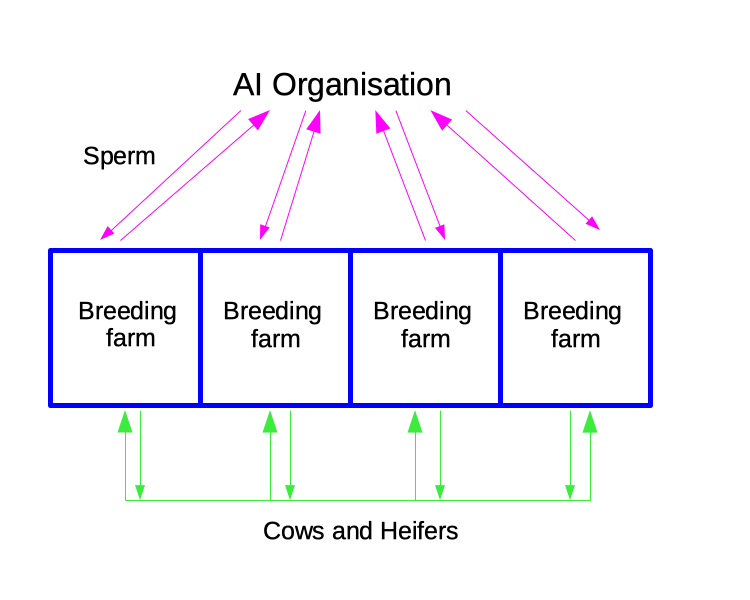
\includegraphics[width=11cm]{odg/monoliticbreedingprogram} \caption{Monolitic Structure of Cattle Breeding Program}\label{fig:monoliticbreedingprogram}
\end{figure}

Monolithic breeding programs (see Figure \ref{fig:monoliticbreedingprogram}) are typically found in cattle and horse breeding organisations. Such structures are often chosen when state subsidies are paid to breeding organisations based on the number of animals in the herdbook. This gives incentive for breeding populations to include all animals in the herdbook. In species like cattle, progeny performance tests require large populations to achieve good test accuracies. Large breeding populations with many herds are easier to be organized in monolithic breeding programs.

\begin{figure}
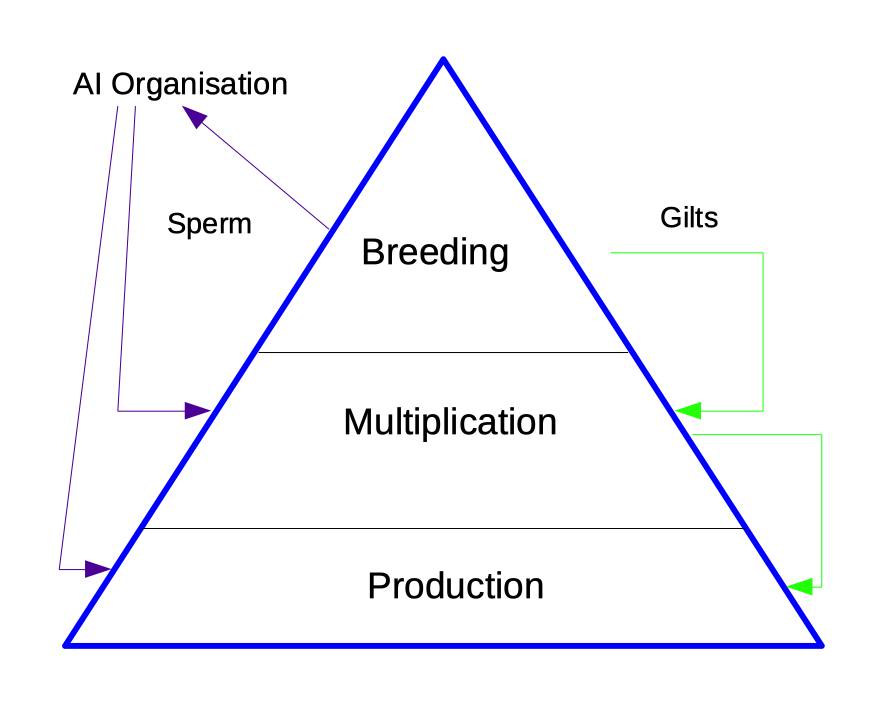
\includegraphics[width=11cm]{odg/hierarchicalbreedingprogram} \caption{Hierarchical Structure of Pig Breeding Program}\label{fig:hierarchicalbreedingprogram}
\end{figure}

Hierarchical structures are more frequently found in pigs and in chicken. Differences are rooted in biology and in economic circumstances. In pigs and in chicken population sizes are high and consequently the monetary value of a single animal is quite low. Performance tests for complete populations would be too expensive. Because pigs and chicken can have a high number of progeny per parent, performance testing and breeding is restricted to a small number of specialized herds. High number of progenies per parent and short generation intervals allow to transmit genetic progress quite rapidly. Cross-breeding to benefit from positive heterosis effects is used extensively in such breeding programs. Figure \ref{fig:hierarchicalbreedingprogram} shows the structure of a hierarchical breeding program in pigs.

In cattle and horse breeding, the situation is different. Single breeding animals can have a very high value. With the low numbers of progeny per parent it is well worth while to have all breeding animals under a performance test and to record as many traits as possible from each animal in the population. Furthermore, most data used for breeding evaluations are also used for management purposes. Hence it is normal that in such populations the vast majorities of the farms are members of a breeding organisation.

\hypertarget{gel-bprog-succbreedprog}{%
\section{Success Of A Breeding Program}\label{gel-bprog-succbreedprog}}

In Figure \ref{fig:bprogdiag} the influential components are shown. All these factors are to be considered when designing and when running a breeding program. The success of a breeding program as measured by the selection response is determined by just four factors which are given in the following formula.

\begin{equation}
\Delta G = \frac{i * r_{TI} * \sigma_T}{L} = \frac{SD}{L}
\label{eq:gel-bprog-selresponse}
\end{equation}

\begin{tabular}{lll}
where  &  &  \\
       &  $i$         &  selection intensity \\
       &  $r_{TI}$    &  accuracy of predicted breeding values \\
       &  $\sigma_T$  &  additive genetic standard deviation \\
       &  $L$         &  generation interval
\end{tabular}

The four determining factors can be modified to change the selection response. The denominator of the fraction in \eqref{eq:gel-bprog-selresponse} is also called selection difference (\(SD\)).

\hypertarget{gel-bprog-selintensity}{%
\subsection{Selection Intensity}\label{gel-bprog-selintensity}}

Selection intensity \(i\) measures the superiority of the selected animals compared to the population mean. Assuming the traits to be normally distributed, the selection intensity can be computed based on the selection boundary. Given a trait which is to be increased by selection, the animals to the right are called the selected animals. Only selected animals will be parents of the next generation. The mean of the selected animals corresponds to the selection difference (SD). Let us assume that the selection boundary \(SB\) is one standard deviation \(\sigma_P\) above the population mean \(M\), hence

\begin{equation}
SB = M + \sigma_P \notag
\end{equation}

According to the laws implied by the normal distribution, this means that about \(16\%\) of the animals are selected. The selection difference (SD) corresponds to \(1.53\), that means the mean of the selected animals is \(1.53\) times the phenotypic standard deviation above the population mean.

The selection intensity \(i\) can be expressed as the selection difference (SD) in units of the phenotypic standard deviation

\begin{equation}
i = \frac{SD}{\sigma_p}
\label{eq:gel-bprog-seltint}
\end{equation}

The selection intensity \(i\) can also be computed only based on the selection boundary. Namely

\begin{equation}
i = \frac{z}{p}
\label{eq:gel-bprog-seltintselbound}
\end{equation}

\begin{tabular}{lll}
where  &  &  \\
       &  $z$         &  density value at selection boundary \\
       &  $p$         &  proportion of animals selected 
\end{tabular}

\hypertarget{gel-bprog-accpredbv}{%
\subsection{Accuracy Of Predicted Breeding Values}\label{gel-bprog-accpredbv}}

The accuracy of the predicted breeding values is measured via the correlation between the true and the predicted breeding values. Intuitively it is clear that predicted breeding values with low accuracies lead to animals selected that are on the wrong side of the selection boundary. The more accurate the predicted breeding value, the lower the probability that the wrong animals are selected.

\hypertarget{gel-bprog-addgenvar}{%
\subsection{Additive-genetic Variance}\label{gel-bprog-addgenvar}}

Selection response is measured on the phenotypic scale, but it actually happens on the genetic scale. The additive-genetic variance determines how much a given phenotype can be changed for a given breeding investment. Low additive-genetic variances can explain why for some traits selection responses are small although large investments are made and breeding values are predicted with high accuracies.

\hypertarget{gel-bprog-genint}{%
\subsection{Generation Interval}\label{gel-bprog-genint}}

The generation interval corresponds to the average age of the parents when their progeny is born. It can be influenced by planning and by the use of biotechnologies. Many practical breeders have problems to find a positive attitude towards shorter generation intervals. Very often short generation intervals are confounded with decreased longevity. The former term is an important parameter which determines the selection response per year. Longevity on the other hand is an important trait that influences the economic profitability of a production herd.

\hypertarget{gel-bprog-fedreg}{%
\section{Federal Regulations}\label{gel-bprog-fedreg}}

Swiss breeding organisations are obliged by federal regulations \citep{Bundesrat2012} to predict breeding values on a regular basis in order to obtain any federal subsidies. Article 1 of the regulation contains the following points

\begin{enumerate}
\def\labelenumi{\alph{enumi}.}
\tightlist
\item
  the recognition of breeding organisations and private breeding companies
\item
  the payment of subsidies
\item
  the payment of subsidies to sustain rare breeds
\item
  the payment of funding for research projects
\item
  the introduction of breeding animals as well as semen, eggs and embryos
\item
  the quotas to import breeding animals and semen
\end{enumerate}

In Article 2 the term \textbf{prediction of breeding values} is defined as an accepted procedure according to currently recognized statistical standards to predict the genetic values of an animal compared to other animals of the same population.

The federal government is planning to revice the regulations to support animals breeding. The plans are based on \citep{Lehmann2018} which contains strategies for livestock breeding in Switzerland.

\hypertarget{gel-implbp}{%
\chapter{Implementation Of A Breeding Program}\label{gel-implbp}}

\hypertarget{gel-implbp-intro}{%
\section{Introduction}\label{gel-implbp-intro}}

In chapter \ref{gel-bprog} (see Figure \ref{fig:bprogdiag}) the different types of breeding programs and the components of a breeding program are shown and described. This chapter aims at giving an outline of how to implement a specific breeding program for a given population. We assume a beef breeding organisation that approaches us and we have to consult them on how to implement a breeding program. The breeding organisation wants to improve their breeding animals with respect to the economic profitability of the animals sold at the production level. This implies that we want to use a hierarchical structure for the breeding program (see Figure \ref{fig:gel-implbp-hier-bp}).

In previous years the beef breeding organisation has included several production and reproduction traits. The traits have been combined into a selection index. The weighting factors of the different traits in the selection index have been determined by the desired gain approach. As shown in section \ref{gel-implbp-desired-gains} index weights determined by desired gains do not reflect the economic context of a production system. But the more recent developments in the agricultural sector with decreasing market prices puts a lot of pressure on the economic efficiency of the production animal goods. Hence, the beef breeding organisation wants to have a better consideration of the economic context of beef production in their breeding goal. As a consequence of that, the breeding organisation agreed on changing the currently used breeding goal to a scientifically formulated breeding goal. In what follows, we briefly describe the desired gain approach and then develop the breeding goal that is based on the economic context of the animal production system.

\begin{figure}[H]
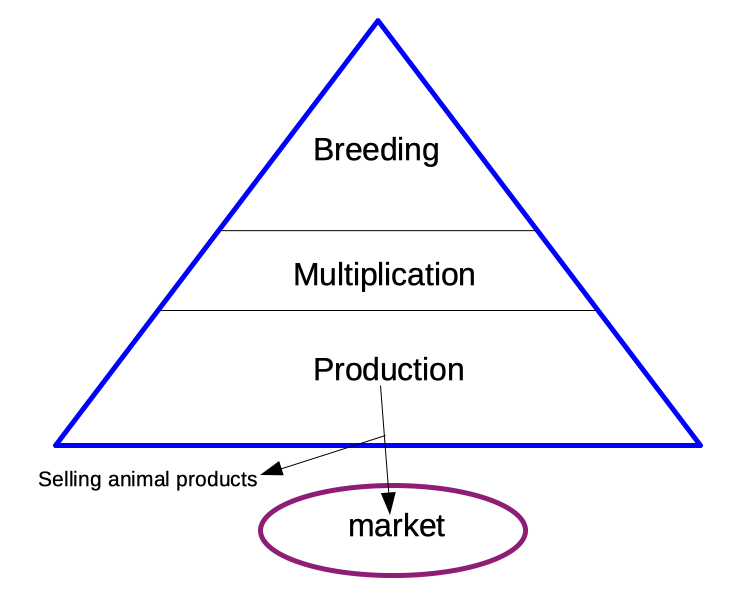
\includegraphics[width=11cm]{odg/gel-implbp-hier-bp} \caption{Hierarchical Structure of a Breeding Program}\label{fig:gel-implbp-hier-bp}
\end{figure}

\hypertarget{gel-implbp-desired-gains}{%
\section{Desired Gains}\label{gel-implbp-desired-gains}}

The desired gains approach is described e.g.~in \citep{Brascamp1984} and in \citep{Gibson1990}. There is a fundamental difference between economic selection indices and restricted or desired gains indices. The term \textbf{restricted} selection index refers to the situation where the genetic change of one or several traits are set to \(0\) whereas in a desired gains index, the genetic change of certain traits is pre-specified. It is also possible to have a mixture of restricted selection indices, desired gains indices and economic indices.

With economic selection indices, the response to selection is entirely determined by the economic weights (also known as economic values) of the traits contributing to the economic merit of the production animals, the phenotypic variance-covariance matrix among the traits in the index, and the genetic covariance between the traits in the index and the traits of economic interest. It has to be noted here, that all traits of economic interest are included in the aggregate genotype (\(H\)).

With restricted and desired gains indices, there are predetermined constraints on genetic response of some traits that partially or completely override the response determined by their economic weights. In the case of restricted indexes, economic weights of restricted traits are not defined. Justification for the use of restricted or desired gains indices has been either that some traits are considered already to be at an economic optimum or that economic weights are difficult or impossible to determine. However, in the former case economic weights at the optimum are by definition zero. It would then be appropriate to use an economic weight of zero or, if there is marked nonlinearity in the economic weights, to use a nonlinear selection index.

Assuming that a given trait is already at its economic optimum, its economic weight would be set to zero. After a given time corresponding to the planning horizon of the breeding program, it must be verified that the trait is still at its economic optimum. It could very well be the case that via correlated selection responses, the trait changes, even if the economic weight of the trait itself is set to zero. In case where the trait is no longer at its economic optimum it would receive automatically an economic weight different from zero such that the trait mean moves back towards its economic optimum. Such an iterative strategy can be used for traits with a certain economic optimum. Examples of such traits are fatness in beef or in pigs.

Hence the previous paragraph shows that it is not really necessary to use the tool of restricted indices or desired gains indices. The use of economic selection indices is fully sufficient even for traits with an intermediate economic optimum.

\hypertarget{gel-implbp-devbg}{%
\section{Development Of The Breeding Goal}\label{gel-implbp-devbg}}

In this section, we focus on the development and the design of a breeding goal that focuses on the economic merit of the production of marketable animal goods. According to \citep{Phocas1998}, three points are to be considered when developing such a breeding goal.

\begin{enumerate}
\def\labelenumi{\arabic{enumi}.}
\tightlist
\item
  description of production system
\item
  modelling the profit for a typical herd
\item
  derivation of economic values
\end{enumerate}

For reasons of simplicity we are assuming that all herds have the same production system. It is important to note here that in a hierarchical breeding program such as shown in Figure \ref{fig:gel-implbp-hier-bp}, the herd described in subsection \ref{gel-implbp-descprodsys} comes from the production sector situated at the bottom of the triangle. The reason for using a herd from the production tier as the basis of the description of the production is that the breeding and possibly the multiplier sections of the breeding program have to adapt their breeding animals to the needs and requirements of the production herds. Looking at the different participants of the breeding program as a client-supplier relationship, the producers are clients of the breeding and the multiplier farms for young production animals. These animals must meet the requirements of the production farms. As a consequence of that the breeding and multiplier farms have to raise young animals that fit the needs of the production farms. This is done by designing the breeding program implemented in the breeding farms according to the needs of the production farms. The implementation of the breeding program must yield tools for the breeding farms to be able to select the best animals as parents. One possibility of such an implementation is shown here for an idealized and simplified situation.

\hypertarget{gel-implbp-descprodsys}{%
\subsection{Description Of Production System}\label{gel-implbp-descprodsys}}

A production system is defined by its required inputs consisting of feed, housing, labor and other fixed costs and by the products (output) that are sold. Furthermore housing systems, feeding regimes and other management components that affect the production costs are important properties of a production system. On the output-side it is important to know what type of markets the animal products can be sold to.

Overall the production system helps us to identify which traits of the animals have an economic impact. Those traits with an economic importance for the production system have to be included in the aggregate genotype.

Figure \ref{fig:gel-implbp-prodsys} illustrates a production system by showing the most important components affecting the profitability of a typical herd.

\begin{figure}
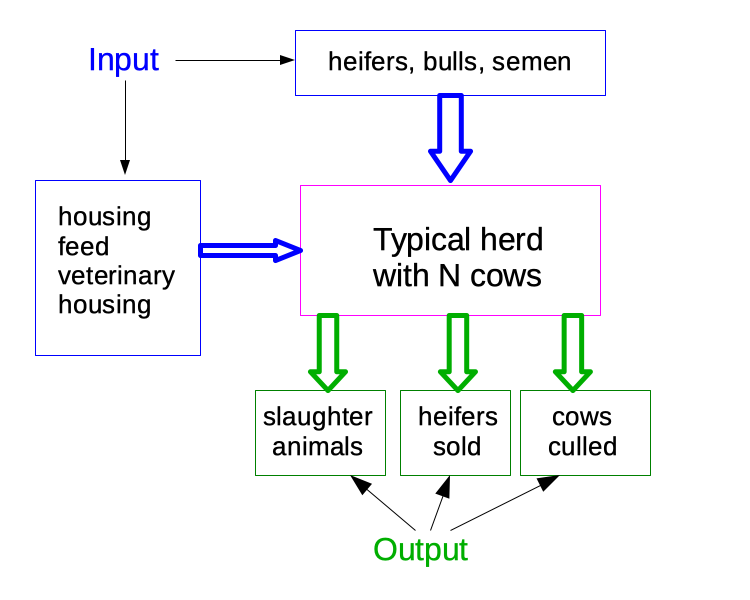
\includegraphics[width=11cm]{odg/gel-implbp-prodsys} \caption{Production system illustrated by a typical herd}\label{fig:gel-implbp-prodsys}
\end{figure}

In our example, the assumed herd has \(N\) cows. Cows are inseminated using artificial insemination. Once a year the cows are expected to produce a calf. The calves are raised, fattened and sold as slaughter animals. From the \(N\) cows each years a proportion of \(0.18\) is culled and is replaced with young heifers which are bought from breeding or multiplier farms. Figure \ref{fig:gel-implbp-demogherd} corresponds to a simplified version of Figure 1 of \citep{Phocas1998}.

\begin{figure}
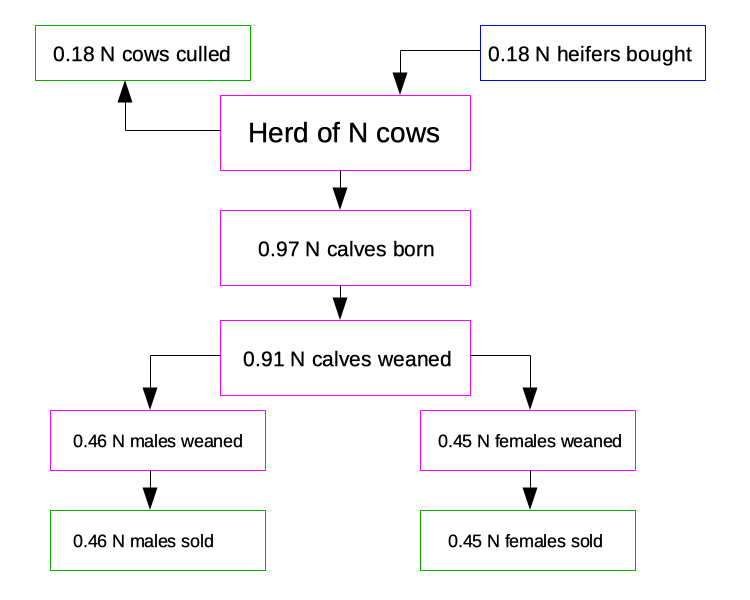
\includegraphics[width=11cm]{odg/gel-implbp-demogherd} \caption{Assumed demography of typical production herd}\label{fig:gel-implbp-demogherd}
\end{figure}

\hypertarget{gel-implbp-dettrint}{%
\section{Determine Traits Of Economic Interest}\label{gel-implbp-dettrint}}

Inputs shown in Figure \ref{fig:gel-implbp-prodsys} generate costs (\(C\)) and Outputs generate revenues (\(R\)). The difference between revenues and costs corresponds to profit (\(P\)) which is the key objective of the whole system that we want to improve. The traits of the animals in the production system which have an influence on the profit of the system are grouped together in the set of the \textbf{economically important} traits. The economically important traits are included in the aggregate genotype which is then used as selection criterion for the breeding animals.

For our example production herd, we are focusing on the carcass performance traits

\begin{itemize}
\tightlist
\item
  carcass conformation (CC)
\item
  carcass fatness (CF) and
\item
  carcass weight (CW).
\end{itemize}

At this stage of our analysis, we are ignoring all traits related to reproduction or survival of calves which are also important for the economic profitability of the production herd. For the moment, we focus on the three traits listed above. This means, we construct the aggregate genotype based on the three traits \emph{CC}, \emph{CF}, and \emph{CW}. The weights of the different traits in the aggregate genotype is the result from the derivation of economic values listed as point 3 of subsection \ref{gel-implbp-devbg}.

\hypertarget{gel-implbp-geneval}{%
\section{Genetic Evaluation}\label{gel-implbp-geneval}}

Once we have determined the traits of economic interest as described in subsection \ref{gel-implbp-dettrint}, we can start to have a look at the genetic part of our analysis of the breeding program. This is done in a genetic evaluation which consists of two parts

\begin{enumerate}
\def\labelenumi{\arabic{enumi}.}
\tightlist
\item
  Variance components estimation
\item
  Prediction of breeding values.
\end{enumerate}

In a practical analysis both parts are using linear mixed effect models with the traits of interest as response variables (\(y\)) and other characteristics as predictor variables (\(x\)). The difference between the two evaluation parts are the results that are of interest. In the first part we are primarily looking for the estimates of the variance components in the model. The second part produces predictions of the breeding values for all breeding animals.

Depending on the number of predictor variables that are available in the dataset that we have available from our breeding organisation, we first have to separate the important predictor variables from the variables that do not have an important effect on the response variable. This separation is done with a preparatory model selection step. In short, we are using all predictor variables available in a fixed linear effects model with the trait of interest as the response variable. Then we are in turn, eliminating the response variable with the smallest impact until a previously chosen model selection criterion is optimized. The remaining set of predictor variables in the optimal model is then used in the linear mixed effects model to estimate variance components and to predict breeding values.

In the chapters that follow, we are having a closer look at how to do the model selection and how to perform the two parts of the genetic evaluation.

  \bibliography{bibliography.bib}

\end{document}
